\chapter{\label{chap:konzeption}Konzeption}
Die erarbeiteten Anforderungen zur Untersuchung der Konfliktmanagementstrategien offlinefähiger Systeme werden in diesem Kapitel für die Konzeption angewendet.\\
Es soll für jede zu untersuchende Technologie ein Prototyp entwickelt werden. Im Rahmen dieser Arbeit entsteht ein Prototyp der \sc{Redux Offline} verwendet und ein zweiter in dem PouchDB und CouchDB eingesetzt wird. Für letzteren könnte genauso gut HOODIE benutzt werden, da HOODIE sowohl PouchDB als auch CouchDB benutzt~\cite{hoodie-how}.
Doch da für den zu entwickelnden Prototyp lediglich diese beiden Komponenten benötigt werden, wurde sich dagegen entschieden.\\
%
Die Wahl viel auf CouchDB und PouchDB, weil diese Technologien häufig in unterschiedlichen Artikeln, die im Zusammenhang mit Offline First Anwendungen stehen, genannt und empfohlen werden.\\
% 
Als einzige Technologie die neben HOODIE, bzw. CouchDB eine Datenbanksynchronisation bereitstellt, stand Realm ebenfalls zur Wahl.
Realm unterstützt jedoch nur die Entwicklung von mobilen Anwendungen und ist außerdem zahlungspflichtig.
Zusätzlich dazu ist der Object Server, der Teil der für die Datensynchronisation zuständig ist, und dessen Dokumentation nicht quelloffen.
Das heißt es ist nicht nachvollziehbar welche der im Realm Whitepaper genannten Konfliktmanagementstrategien, \gls{OT} oder \gls{LWW}, angewandt wird.
Bei Betrachtung der von Realm voreingestellten Regeln, dass Löschungen und jede letzte Aktualisierung immer gewinnen, ist kein herausstechender Synchronisationsalgorithmus zu erkennen.\\
% 
Aus diesen Gründen wurde als Alternative zu Realm Redux Offline gewählt. Redux ist ein mächtiges und oft verwendetes Tool ist, was sowohl in mobilen, als auch Desktopapplikationen integriert werden kann.
Die Versprechungen von Redux Offline sind hoch und es soll untersucht werden, inwiefern diese eingehalten werden.\\
% 
% 
% 
Bis zu einem gewissen Status, nämlich dem der Verwendung der Technologien, sind beide Prototypen -- bis auf den Namen-- identisch.
% Beginnend mit dem Aufbau der exemplarischen Anwendung werden in den folgenden Abschnitten die  der Anwendungsaufbau, Architektur  und schließlich \todo{blabla} die graphische Oberfläche aufgeführt.
% Den Raum aller möglichen Lösungen anhand der Anforderungen auf die in irgendeinem Sinn beste / geeignetste einzuschränken:\\
% App entwickeln, in der es einen `Verbindung unterbrechen` Knopf gibt ', oder ob es aus irgendwelchen Erwägungen notwendig sein könnte, das über eine separate Instanz zu machen.
%
% Aufbau
%
\section{\label{chap:aufbau}Anwendungsaufbau}
Die Prototypen bestehen im Frontend aus React und wurden mit \sc{Create React App} erstellt. \sc{Create React App} erstellt ein Projekt mit dem gewünschten Namen, generiert eine initiale Projektstruktur (vgl. \autoref{fig:init}) und installiert die dafür benötigten Abhängigkeiten~\cite{create-react}.
\begin{figure}[H]
  \centering
  \begin{subfigure}[t]{0.4\textwidth}
          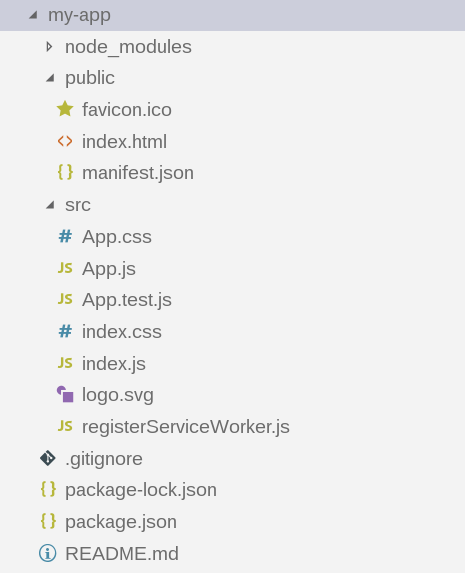
\includegraphics[width=\textwidth]{Ordnerstruktur}
          \caption{Die initiale Projektstruktur}
          \label{fig:init}
  \end{subfigure}
  ~
  \begin{subfigure}[t]{0.4\textwidth}
          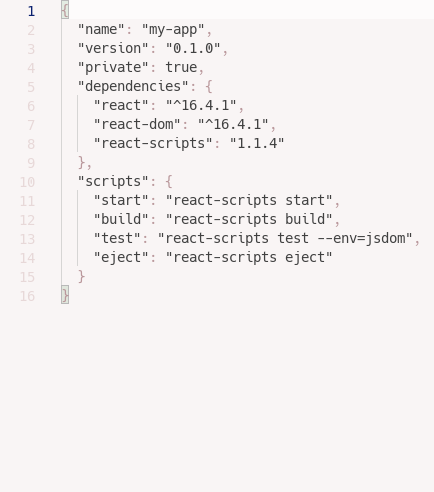
\includegraphics[width=\textwidth]{rca-package}
          \caption{Die initiale package.json Datei}
          \label{fig:init2}
  \end{subfigure}
  \grayRule
  \caption[Create React App: initiale Testapplikation]{einer mit Create React App erstellten Testapplikation}
  \label{fig:create-react-app}
\end{figure}
%
Diese sind im Verzeichnis node\_modules installiert.
Außerdem ist ein ServiceWorker enthalten der die \gls{Assets} cacht.
Als Template gibt es nun die \tt{public/index.html}-- Datei. In der \tt{index.js}--Datei werden die React--Komponenten und der ServiceWorker initialisiert.
Alle \tt{App.*}--Dateien umfassen eine minimale Beispielanwendung.
In der generierten \tt{package.json}--Datei (vgl. \autoref{fig:init2}), befinden sich Informationen über die Anwendung und ihre Abhängigkeiten. Im Unterpunkt \tt{scripts} werden Kommandozeilen-Aufrufe definiert und können mit dem Befehl \tt{npm run} aufgerufen werden.
%
% React Komponenten
%
\sub{Aufbau der React Komponenten}
React ist eine Open--Source--Bibliothek, die dazu dient, die Viewkomponente des Model-View-Controller-Ansatzes abzudecken, also die Seite der Anwendung, die für die Anzeige und Interaktion zuständig ist.
Ein Vorteil von React sind die komponentenbasierte Philosopie. Eine Komponente ermöglicht die Aufteilung der \gls{UI} in kleine Teile und ist eine abstrakte Basisklasse. Einmal implementiert, lässt sich eine Komponente immer wieder verwenden~\cite{react}.\\
%
Eine Komponente kann einen internen State besitzen, oder die Daten aus den \tt{props} nehmen.
\tt{Props} sind Daten, die von der Elternkomponente übergeben werden und können auch nur von dieser manipuliert werden.
Eine React--Komponente hat immer eine \tt{render()}--Funktion, die die Daten aus dem State oder den \tt{props} liest und zurückgibt, was dargestellt werden soll.
Hier wird das zur Komponente gehörende \gls{HTML} erzeugt. Jede Änderung des States führt einen erneuten Aufruf der \tt{render()}--Funktion mit sich.\\\\
%
%
React--Komponenten können in zwei Kategorien aufgeteilt werden, Containerkomponenten und Viewkomponenten.
Containerkomponenten dienen als Datenquelle und in ihnen steckt die Logik wie etwas funktioniert.
Sie stellen außerdem Callbackfunktionen für die Viewkomponenten bereit.
Viewkomponenten haben keine andere Zuständigkeit als die Daten, die sie über ihre \tt{props} erhalten, anzuzeigen und ggf. die ebenfalls empfangenen Callbackfunktionen aufzurufen ~\cite{react-components}.\\
Zur Veranschaulichung wird anhand des Listings \ref{code:react-form} eine beispielhafte Containerkomponente, und im \autoref{code:react-form-view} die dazugehörige Viewkomponente beschrieben.
Zusammen repräsentieren sie ein Formular, in dem der Name des Kontakts angezeigt und geändert werden kann.
%
\begin{center}
  \lstinputlisting[language=REACT,
  numbers=left,xleftmargin=20pt,framexleftmargin=15pt,
  firstline=1, lastline=22,
  caption={Eine React Containerkomponente},
  label=code:react-form]{code/Form.js}
\end{center}
%
Die Formular--Containerkomponente hat ein Kontaktobjekt im internen State gespeichert.
Auf dieses Objekt haben andere Komponenten keinen Zugriff und es ist nur via \tt{setState()} änderbar.
Initial wird das Kontaktobjekt über die \tt{props} in Zeile 5 geladen. So kann das Vorausfüllen der Eingabefelder realisiert werden.\\
In Zeile 9 steht die \tt{handleChange}--Funktion, die den internen State in Zeile 12 mit den eingegebenen Werten aktualisiert.
Eine Viewkomponente wird wie in in den Zeilen 17 bis 19 eingebunden. Ihr wird der interne State übergeben, also das Kontaktobjekt und die \tt{handleChange}--Funktion. 
Die beiden Parameter sind in Zeile 1 des folgenden Listings wiederzufinden.
% listing
\begin{center}
  \lstinputlisting[language=REACT,
  numbers=left,xleftmargin=20pt,framexleftmargin=15pt,
  firstline=24, lastline=33,
  caption={Eine React Viewkomponente},
  label=code:react-form-view]{code/Form.js}
\end{center}
%
Die Viewkomponente macht nichts anderes, als die ihr übergebenen Daten anzuzeigen.
Im Ereignisbehandler des Eingabefeldes wird die übergebene \tt{handleChange}--Funktion in Zeile 5 aufgerufen.
Diese Komponente besitzt keinerlei Logik.
%
% Redux
%
\sub{Verwendung von Redux Offline}
Redux Offline kann nur zusammen mit Redux verwendet werden, eine Bibliothek die in \autoref{chap:redux} vorgestellt wird.
Deswegen ist für diesen Prototypen die Implementierung von Redux vorausgesetzt.\\\\
%
Redux Offline ist eine erweiternde Bibliothek für Redux, dessen Funktionsweise in Abschnitt \ref{sub:reduxoffline} detailliert beschrieben wird.\\
Nach der Installation muss der Redux \tt{store} zusammen mit dem \tt{offline "-store "-enhancer} erzeugt werden. Listing \ref{code:store} visualisiert diesen Vorgang. Ein Redux \tt{store} wird mit dem \tt{storeCreator} in Zeile 5 erzeugt. Ein \tt{store "-enhancer} ist eine Funktion, die den \tt{storeCreator} neu zusammenfügt und einen neuen, erweiterten \tt{storeCreator} zurückgibt.
Redux Offline kommt mit einer Grundkonfiguration (siehe Zeile 3). Diese wird dem \tt{offline store enhancer} in Zeile 8 übergeben.
%
\begin{center}
  \lstinputlisting[language=REACT,
  firstline=50,lastline=62,
  numbers=left,xleftmargin=20pt,framexleftmargin=15pt,
  caption={Erstellen eines Stores mit Redux Offline},
  label=code:store]{code/Redux.js}
\end{center}
%
Der gesamte Kontext, der zum Synchronisieren einer Aktion erforderlich ist, ist in einem zusätzlichen Metaattribut gespeichert.
Damit die Anwendung weiß, wie die Aktionen verarbeitet werden sollen, wird sie mit dem Metafeld dekoriert.
Die Aktion zum Lesen der Kontakte könnte dann wie im folgenden Listing aussehen.
%
\begin{center}
  \lstinputlisting[language=REACT,
  firstline=9,lastline=20,
  numbers=left,xleftmargin=20pt,framexleftmargin=15pt,
  caption={Aktion \tt{fetchContacts} mit Metaattribut},
  label=code:react-meta]{code/Redux.js}
\end{center}
%
Das erste \tt{meta.offline}--Feld beschreibt die Netzwerkaktion, die ausgeführt werden soll, also den Aufruf an die angegebene URL in Zeile 6.
Bei \tt{commit} in Zeile 7 wird festgelegt welche Aktion bei erfolgreichem Netzwerkaufruf ausgeführt werden soll.
Für den Fall, dass von dem angefragtem \gls{API} ein 4xx oder 5xx \gls{HTTP}--Statuscode zurückkommt, wird die im \tt{rollback} definierte Aktion gefeuert ~\cite{redux-offline-npm}.\\
Die Aktionen beschreiben nur was passiert. Wie der Status sich ändert, wird im Reducer beschrieben.
Das Listing \ref{code:reducer} illustriert, wie das prototypisch umgesetzt werden könnte.
%
\begin{center}
  \lstinputlisting[language=REACT,
  firstline=36,lastline=50,
  numbers=left,xleftmargin=20pt,framexleftmargin=15pt,
  caption={Reducer mit allen Aktionen die im Metafeld beschrieben werden},
  label=code:reducer]{code/Redux.js}
\end{center}
%
In den Zeilen 6 bis 8 ist nachzulesen, wie sich der \gls{App}status bei erfolgreichem Netzwerkaufruf aktualisiert.
Der Status aktualisiert sich nur, wenn sich die Antwort vom Server von diesem unterscheidet.
%
%
% Architektur
%
\section{Architektur}
Die zu erstellenden Prototypen erhalten die Namen \it{amilia-qouch} und \it{amilia-rdx}, wobei Amilia der Name ist, der sich in den Beispielkontakten in den Szenarien wiederfindet.
Die Abkürzung \it{rdx} steht für Redux und zeigt, dass dieser Prototyp Redux Offline verwendet.
Die Endung \it{qouch} soll das Zusammenspiel von CouchDB und PouchDB darstellen. Der Buchstabe Q klingt wie das hart ausgesprochene C in Couch und wenn man das kleine Q horizontal spiegelt, sieht man das P für Pouch.\\\\
%
%
Beide Prototypen setzen sich aus den nachfolgend beschriebenen Komponenten zusammen, welche in \autoref{fig:uml} veranschaulicht werden.
Die Abbildung stellt ein Komponentendiagramm dar.
Es handelt sich hierbei nicht um das UML Komponentendiagramm, sondern um ein eigens entworfenes.
Die Bezeichnung ist durch die Darstellung von React--Komponenten begründet.\\\\
%
%
Jeder Kasten repräsentiert eine Komponente, deren Bezeichnung im Kopf steht.
In dem Teilbereich darunter sind der State oder die Props der Komponente abzulesen. Bei Containerkomponenten handelt es sich um den Status. Die Viewkomponenten haben keinen eigenen State, bei Ihnen stehen an dieser Stelle die Props.\\
Alle Komponenten, bei denen im Namen das Wort ''Container'' vorkommt, sind Containerkomponenten, beinhalten Logik und entscheiden welche Viewkomponente gerendert wird.
Die anderen sind Viewkomponenten und können im Gegensatz zu den Containerkomponenten den Appstatus nicht manipulieren.
Sie können nur die von der Elternkomponente durchgereichten Funktionen aufrufen.
Anhand der Linien ist abzulesen auf welche Funktionen und Eigenschaften die Viewkomponenten Zugriff haben.
Kursiv geschriebene Werte kennzeichnen externe Module, die von der Komponente verwendet werden.
Es werden für jede Komponente, bis auf ''Contacts'', nur die eigens implementierten Funktionen aufgelistet. Um besser nachvollziehen zu können, welche Funktionen und Eigenschaften von der Contacts--Komponente an die Kindkomponenten durchgereicht werden, werden diese in grauer Schrift aufgezählt.
%
% \begin{figure}[H]
%   \centering
%   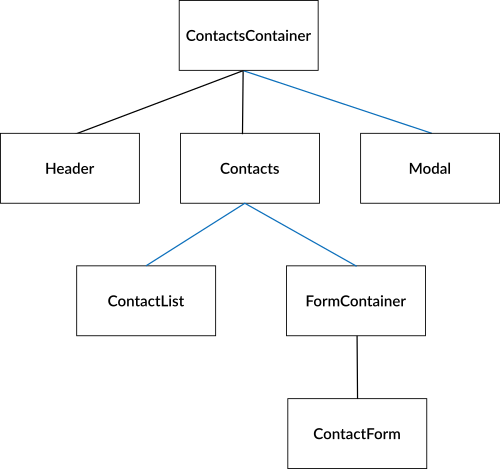
\includegraphics[width=0.8\textwidth]{umlsimple}
%   \grayRule
%   \caption[Komponentendiagramm]{Komponentendiagramm der Prototypen}
%   \label{fig:umlsimple}
% \end{figure}
\begin{figure}[H]
  \centering
  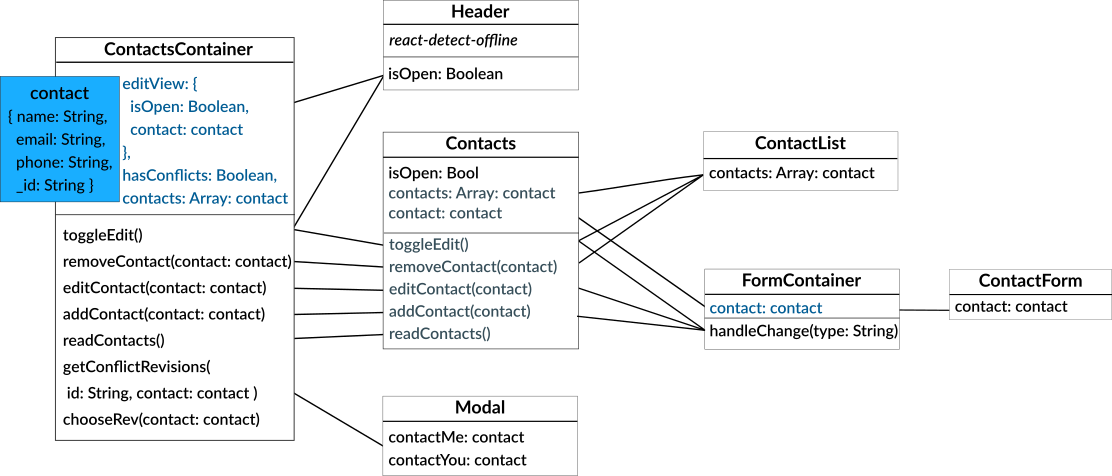
\includegraphics[width=\textwidth]{uml2}
  \grayRule
  \caption[Komponentendiagramm]{Komponentendiagramm der Prototypen}
  \label{fig:uml}
\end{figure}
%
%
Die Komponente \tt{ContactsContainer} ist das Herzstück der Anwendung.
Hier wird die graphische Oberfläche definiert und es werden alle notwendigen Funktionen bereitgestellt.
Die Komponente hat einen internen State in dem sowohl die Kontaktliste, als auch die Daten für das Formular gespeichert sind.
Im Diagramm ist der Status an der blauen Schrift zu erkennen.
Das Objekt \tt{editView} speichert den im Formular zu ladenden Kontakt und zeigt welche Ansicht gerade aktuell ist.
Ist das Attribut \tt{isOpen} auf \tt{true} gesetzt, wird das Formular gerendert, andernfalls die Kontaktliste.
Wie das Kontaktobjekt aufgebaut ist, zeigt der blaue Kasten im Diagramm.
Wird eine Aktion zum Ändern der Ansicht aufgerufen, beispielsweise durch das Betätigen eines Knopfes, wird über die Funktion \tt{toggleEdit()} der interne State aktualisiert, wodurch ein erneutes Rendern der Komponente eingeleitet wird. Dann wird entsprechend die Liste oder das Formular gerendert.\\
%
Der \tt{Header} implementiert das externe Modul \tt{react-detect-offline} und kann so den Netzwerkstatus anzeigen.
Die Komponente hat Zugriff auf die \tt{toggleEdit}--Funktion und einen Knopf, der an diese gebunden ist.
Damit kann das Rendern des Kontaktformulars eingeleitet werden.
Dieser Knopf soll nur angezeigt werden, wenn die Liste aktiv ist. Diese Information ist in dem Attribut \tt{isOpen} abzulesen.\\
Die \tt{ContactList} repräsentiert die Kontaktliste und wird initial gerendert. Hier werden alle Kontakte als Liste dargestellt.
Das Bearbeiten kann durch den Aufruf der durchgereichten Funktion \tt{toggleEdit()} eingeleitet werden.
Durch den Aufruf von \tt{remove"-Contact()} wird der Kontakt gelöscht.\\
%
Die Komponente \tt{Contacts} gehört als Viewkomponente zu \tt{ContactsContainers}. Je nach Wert des Attributs \tt{isOpen}, wird hier entweder die Kontaktliste oder das Formular gerendert. Die restlichen, grau geschriebenen Eigenschaften und Methoden werden an die Kondkomponenten durchgereicht.\\
%
Die Komponente \tt{ContactForm} zeigt, sofern vorhanden, alle im Kontakt gespeicherten Daten an.
Gibt es keine Kontaktdaten, die geladen werden können, kann ein neuer Kontakt angelegt werden.
In der View, dem \tt{ContactForm}, gibt es zum Hinzufügen und Bearbeiten des Kontakts Eingabefelder für den Namen, die E-Mail und die Telefonnummer des Kontakts.
Zusätzlich zu den Eingabefeldern für jedes Kontaktattribut hat sie zwei Knöpfe, mit denen die Aktion bestätigt oder abgebrochen werden kann.\\
Der dazugehörige Ereignisbehandler befindet sich im \tt{FormContainer}. 
Der ''lauscht'' auf die Veränderung der einzelnen Eingabefelder und speichert alle Änderungen in einer Kopie des Kontakts im internen State.
Wird die Aktion durch den entsprechenden Knopf bestätigt, wird die Kopie des Kontakts an \tt{Contacts} gegeben und dort entweder via \tt{addContact()} hinzugefügt oder via \tt{editContact()} bearbeitet.
Wenn die Aktion abgebrochen wird, ruft der \tt{FormContainer} die \tt{toggleEdit()} Funktion in der Hauptkomponente auf.\\\\
%
%
Kommt es beim Hinzufügen, Bearbeiten oder Löschen eines Kontakts zum Konflikt, werden mittels \tt{getConflictRevisions()} die beiden Versionen des konfliktbehafteten Kontakts ermittelt.
Der Kontakt wird dann in beiden Varianten, der alten und der neueren Version, an einen Konfliktdialog übergeben, der sich prompt öffnet.
Dieser hat Zugriff auf die Funktion \tt{chooseRev} in der \tt{Contacts}--Komponente.
Der Dialog hat pro Kontakt einen Knopf. Jeder dieser Knöpfe ruft auf Klick die \tt{ChooseRev}--Funktion mit dem ausgewähltem Kontakt als Parameter auf.
Innerhalb von \tt{chooseRev} wird der übergebene Kontakt gespeichert und die konkurrierende Version verworfen.\\\\
%
% BACKEND
%
Eine Backendimplementierung ist für den Prototypen \it{amilia-qouch} nicht notwendig, da dies bereits durch die Verwendung von CouchDB gegeben ist.
Die \autoref{fig:qouch-model} skizziert die Architektur von \it{amilia-qouch}.
% TODO:
Die Containerkomponenten handhaben die Daten, die in den Viewkomponenten angezeigt werden und speichert sie in PouchDB.
PouchDB synchronisiert sich mit der CouchDB und schreibt die Daten zurück in das Model.
% Client - Server - Modell
\begin{figure}[H]
  \centering
  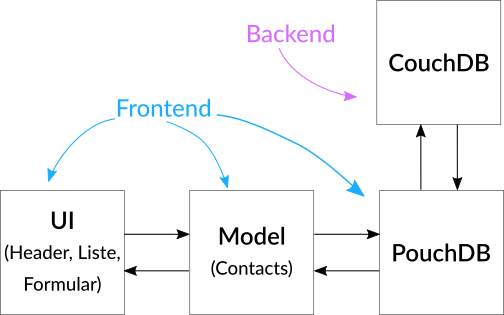
\includegraphics[width=0.8\textwidth]{qouch-model}
  \grayRule
  \caption{Client-Server-Modell des Prototypen \it{amilia-qouch}}
  \label{fig:qouch-model}
\end{figure}
%
Obwohl Redux Offline nach eigener Aussage die Datenbank ersetzt~\cite{redux-offline}, stellt es keine Serverdatenbank zur Verfügung.
Deswegen wird ein Node--Server erstellt, der alle \gls{CRUD} Operationen unterstützt.
Die Kontakte werden in einer \gls{JSON}--Datei persistiert.\\
Die \autoref{fig:rdx-model} zeigt, dass der Redux Store in \it{amilia-rdx} PouchDB in \it{amilia-qouch} ersetzt.
Dabei handelt es sich um den Redux Store, der dank Redux Offline alle Daten in einer lokalen Datenbank speichert.
Die im \it{amilia-qouch} verwendete CouchDB wird durch den Server und einer \gls{JSON}--Datei ersetzt.
%
\begin{figure}[H]
  \centering
  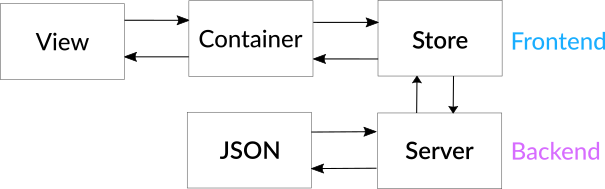
\includegraphics[width=0.8\textwidth]{rdx-model}
  \grayRule
  \caption{Client-Server-Modell des Prototypen \it{amilia-rdx}}
  \label{fig:rdx-model}
\end{figure}
% 
Der Datenfluss ist derselbe wie im Model des Prototyps \it{amilia-qouch}, mit dem Unterschied, dass der Store und der Server sich nicht automatisch synchronisieren.
Der Store schickt zwar automatisch die Daten an den Server sobald er mit dem Internet verbunden ist, aber in die andere Richtung ist das nicht implementiert.
Deswegen werden nach jeder Aktion die Kontakte vom Server geladen.
% Todo: werden nur die geladen die es noch nicht gibt? 
%
% Speicherung & Sync
%
\sub{\label{chap:persist}Das Speichern der Daten}
Das Seichern von Kontakten wird in den Prototypen unterschiedlich implementiert.
%
% --------------------------------------------------------------------------------- Qouch
%
\subsub{Daten mit PochDB und CouchDB speichern}
Für den Protoyp \it{amilia-qouch} muss zunächst CouchDB installiert werden.
% sudo apt-get install couchdb
Sobald dieser Schritt erledigt ist läuft CouchDB auf \tt{localhost:5984} und ist einsatzbereit.
Das asynchrone \gls{API} von PouchDB stellt alle notwendigen Funktionen bereit die sowohl Callbacks, Promises als auch asynchrone Funktionen unterstützen. 
Das Listing \ref{code:pouch} führt alle benötigeten Funktionen auf und zeigt die notwendigen Schritte zur Synchronisation der lokalen PouchDB und CouchDB.\\
Die lokale Datenbank wird in Zeile zwei erstellt. Wenn es die Datenbank mit dem Namen `contacts` bereits gibt, wird sie gestartet.\\
Um eine CouchDB Instanz zu erzeugen ist der Aufruf in Zeile drei mit der URL zur Couch"-DB--Datenbank notwendig. Auch hier erstellt PouchDB die Datenbank, sofern sie noch nicht existiert. PouchDB funktioniert nun als Client zu einer online CouchDB Instanz.
Zur kontinuierlichen Synchronisation beider Instanzen, der lokalen PouchDB und der Couch"-DB, ist lediglich der Aufruf in Zeile fünf erforderlich. Im optionalen Parameter können zum Beispiel FIlter oder Einstellungen zum wiederholten Synchronisationsversuch im Falle eines Fehlschlags gesetzt werden ~\cite{pouch_options}.\\
% GET
Der Aufruf \tt{localDB.allDocs()} in Zeile acht fragt alle in der lokalen Datenbank gespeicherten Kontakte an.
Ohne den Parameter \tt{include\_docs: true} werden nur die ID, \tt{\_id} und die Revisionsnummer, \tt{\_rev} eines jeden gespeicherten Kontakts zurückgegeben.
Ist die Option \tt{conflicts} auf \tt{true} gesetzt, werden Konfliktinformationen zu jedem Kontakt gespeichert. Alle konfliktbehafteten Kontakte haben nun ein \tt{\_conflicts} Attribut. Dort bedindet sich eine Liste mit allen konkurrierenden Revisionen.\\\\
%
Für die nachfolgenden Aufrufe gibt es mehrere Varianten. Eine Anleitung zu dem Umgang mit Konflikten in der PouchDB Dokumentation empfiehlt für das Erstellen, Aktualisieren und Löschen eines Dokuments das Modul PouchDB Upsert zu verwenden. Das wird in Zeile eins zu, PouchDB Objekt hinzugefügt. Jedes Mal wenn eine der \gls{CRUD} Operationen auf einem Dokument ausgeführt wird und das \gls{API} eine Revision verlangt, kann ein Konfliktfehler geworfen werden. Zum praktischen Umgang empflieht PouchDB die Aktion zu wiederholen, bis sie erfolgreich war.
Dazu kann PouchDB Upsert verwendet werden. Es fügt ein neues Dokument hinzu wenn noch keins existiert und aktualisiert es, wenn es vorhanden ist ~\cite{pouch_conflicts}. Konflikte treten so trotzdem auf und CouchDB wählt eine gewinnende Version aus. Alle Konflikte werden immenrnoch gespeichert und die beteiligten Dokumente können wie oben beschrieben aus der CouchDB geladen werden.\\
%
\begin{center}
  \lstinputlisting[language=REACT,
  numbers=left,xleftmargin=20pt,framexleftmargin=15pt,
  caption={Persistierung der Daten mit PouchDB und CouchDB}, 
  label=code:pouch]{code/Pouch.js}
\end{center}
%
% CREATE
Die Zeilen 13 bis 16 zeigen wie ein Kontakt erzeugt werden kann. Bevor das geschieht wird eine ID erstellt die aus dem aktuellen Zeitstempel besteht. Diese wird dann per PouchDB Upsert in dem neuen Dokument gespeichert.\\
% Bei dessen Verwendung wird \tt{\_id} von PouchDB automatisch generiert. Diese Variante wird jedoch nicht empfohlen, weil dann die IDs zufällig sind, die Objekte nicht danach sortiert werden können~\cite{pouch-create}.\\
% UPDATE
Das Aktualisieren eines Kontakts sieht sehr ähnlich aus, da die \tt{upsert} Funktion für beide Operaktionen verwendet wird.
% Zuerst wird der entsprechende Kontakt wie in Zeile zwölf aus der Datenbank angefragt um dann in der Datenbank aktualisiert zu werden.
Mit jedem Update bekommt ein Kontakt von PouchDB eine neue Revision.\\
% DELETE
Man kann einen Kontakt mit PouchDB Upsert wie in Zeile 35 löschen.
Der Kontakt nicht wirklich gelöscht sondern wird durch ein \tt{\_deleted} Attribut als solches markiert.
%Dann ist das Kontaktdokument mit all seinen Feldern gelöscht. Die lokale Datenbank soll sich mit CouchDB synchronisieren. Ist die Revision eines gelöschten Kontakts nicht mehr vorhanden, kann diese nicht repliziert werden. Deswegen wird der Kontakt wie in Zeile 19 als gelöscht markiert und aktualisiert.
%
% Redux Offline
%
\subsub{Daten mit Redux Offline speichern}
Die Idee hinter Redux Offline ist, dass der Redux Store die lokale Datenbank ersetzt. Sobald der Appstatus sich ändert, also irgendwo im Code \tt{setState()} ausgeführt wird, wird er automatisch lokal gespeichert. Dazu wird intern \tt{redux-persist} benutzt, dessen Funktionsweise in Abschnitt \ref{sub:reduxpersist} erläutert wird. Der Redux Store wird bei jeder Änderung persistiert und beim Start der Anwendung neu geladen.
% Es bedarf keiner zusätzlichen Implementierung für die lokale Speicherung der Kontaktdaten.\\
Wie die Daten mit Redux Offline gespeichert synchronisiert werden ist am folgenden Listing erklärt.
\begin{center}  \lstinputlisting[language=REACT,
  numbers=left,xleftmargin=20pt,framexleftmargin=15pt,
  caption={Speicherung der Daten mit Redux Offline}, 
  label=code:syncrdx]{code/Redux-sync.js}
\end{center}
%
Mit dem Aufruf der Aktion ADD\_CONTACT wird der Vorgang gestartet einen Kontakt hinzuzufügen. Die anzufragende URL ist im \tt{meta.offline.effect} Feld in Zeile neun festgelegt. Die Anfrage geht an den Server, welcher die Daten in der \gls{JSON} Datei persisitiert.
Der Reducer hat Zugriff auf das Aktionsobjekt. Dort ist der gerade hinzugefügte Kontakt gespeichert. Mit diesem wird in Zeile 23 der Appstate aktualisiert und so lokal gespeichert.\\
Ist die Netzwerkanfrage erfolgreich, wird die Aktion \tt{commit} in Zeile zwölf gefeuert. Die wird im Reducer in Zeile 25 behandelt. Der \tt{state} wird mit der Antwort vom Server aktualisiert und die Synchronisation ist vollzogen.\\\\
Wie die Serverimplementierung für den gerade beschriebenen Fall aussehen könnte, beschreibt das Listing \ref{code:server}.
%
\begin{center}  \lstinputlisting[language=REACT,
  numbers=left,xleftmargin=20pt,framexleftmargin=15pt,
  caption={Mögliche Serverimplementierung für das Hinzufügen eines Kontakts}, 
  label=code:server]{code/Server.js}
\end{center}
%
In Zeile zwei werden die Kontakte aus einer \gls{JSON} Datei geladen. Diese sind als Objekt in einem Array gespeichert. Bekommt der Server eine post--Anfrage, wird ein Kontaktobjekt mitgesendet. Dieser wird in Zeile fünf in einer Variable zwischengespeichert. 
Wird der Kontakt korrekt gesendet wird er in Zeile zehn dem Array hinzugefügt. Andererseits sendet der Server den \gls{HTTP}--Statuscode 400 an den Client. % bad request
Außerdem wird mithilfe des in Node integriertem Dateisystem\footnote{siehe hierzu: \url{https://nodejs.org/api/fs.html}} Moduls die \gls{JSON} Datei neu geschrieben. Nun ist der neue Kontakt persistiert. Kommt es beim Schreiben der Datei zu keinem Fehler, sendet der Server den frisch gespeicherten Kontakt zurück an den Client.
% -----------------------------------------------------------------------------
%
% Online / Offline
%
\sub{Verbindungsstatus feststellen und ändern}
Für die Überprüfung der Verbindung zum Server wird das Modus \sc{React Detect Offline} verwendet. Es beobachtet den Online-- und Offlinestatus und bietet zwei Komponenten entsprechend des Status den Inhalt rendern. Der folgende Codeausschnitt zeigt eine Verwendung dieser beiden Komponenten. Ist die Anwendung online, wird `you are online` gerendert. Im anderen Fall ~`you are offline`.
%
\begin{center}
\lstinputlisting[language=REACT,caption={Beispiel einer React Detect Offline Implementierung}, label=code:react-detect]{code/Header.js}
\end{center}
%
Das Modul fragt alle fünf Sekunden die URL \url{https://ipv4.icanhazip.com} ab und rendert je nach Verbindungsstatus die entsprechende Komponente. Verschiedene Parameter wie die URL oder das Poll--Interval können konfiguriert werden~\cite{react-detect}.\\\\
%
Der Verbindungsstatus kann im Browser geändert werden. Die Prototypen, die im Rahmen dieser Arbeit entwickelt werden, sollen in den Browsern Firefox und Chromium laufen.\\
In Firefox lässt sich der Netzwerkstatus über das Einstellungsmenü ändern. Dort kann man entweder unter dem Punkt `Sonstiges` oder dem Punkt `Web-Entwickler` `Offline arbeiten` auswählen und ist vom Internet getrennt. Dieser Status lässt sich über den selben Weg rückgängig machen.\\
In Chrome öffnet man dazu die Entwicklertools, geht auf `Netzwerk` und klickt auf die Checkbox `Offline` am oberen Rand. Dieselbe Checkbox ist auch im `Application`--Tab unter `Service Workers` zu finden.
%
% UI
%
\section{Die graphische Oberfläche}
Aus den minimalen Anforderungen an die graphische Oberfläche ergibt sich das Design.
Anhand der folgenden Abbildungen werden die gefertigten Entwürfe der BenutzerInnenoberfläche dargestellt.\\\\
Diese Listenansicht in Abbildung \ref{fig:list} besteht aus dem Header / Kopf und den Listeneinträgen.
Sie zeigt die Kontakteinträge in beiden Netzwerkstatus: online (Abbildung \ref{fig:list-online}) und offline (\ref{fig:list-offline}).\\\\
%
%
Im Header ist abzulesen, ob die Anwendung gerade eine Verbindung zum Server hat oder nicht.
Für eine bessere Prägnanz wurden hierzu unterstützend die Farben Rot für keine Verbindung und Grün für eine bestehende Netzwerkverbindung gewählt.
Rechts im Header gibt es einen Knopf, mit dem man in die Ansicht gelangt, in der ein Kontakt hinzugefügt werden kann.\\
%
In der Liste sieht man die Namen der Person und jeweils einen Knopf zum Bearbeiten oder Löschen.
Mit der Betätigung des ''Delete''--Knopfes wird der entsprechende Eintrag in der Liste gelöscht
\begin{figure}[H]
  \centering
  \begin{subfigure}[t]{0.49\textwidth}
          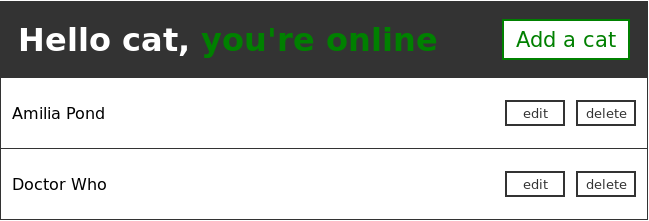
\includegraphics[width=\textwidth]{list-online}
          \caption{Kontaktliste im Onlinestatus}
          \label{fig:list-online}
  \end{subfigure}
  ~ 
  \begin{subfigure}[t]{0.49\textwidth}
          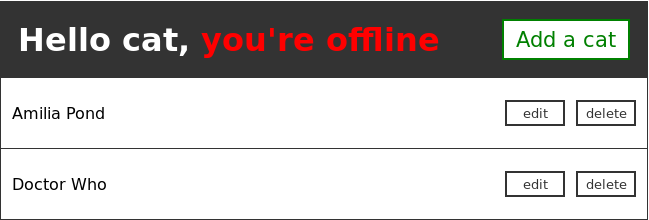
\includegraphics[width=\textwidth]{list-offline}
          \caption{Kontaktliste im Offlinestatus}
          \label{fig:list-offline}
  \end{subfigure}
  \grayRule
  \caption{Die Kontaktliste in beiden Netzwerkstatus}
  \label{fig:list}
\end{figure}
Klickt man auf den Knopf zum Bearbeiten oder auf den zum Hinzufügen eines Kontakts, gelangt man in die Bearbeitungsansicht (vgl. Abbildung \ref{fig:edit}). Der Header ist bis auf den Knopf zum Hinzufügen eines Kontakts identisch zu dem der Liste. Auch hier ist abzulesen, ob die Anwendung on-- oder offline ist. Da man sich bereits in der Ansicht zum Anlegen oder Editieren eines Kontaks befindet, ist der Knopf im Header überflüssig.\\
Ein Kontakt hat einen Namen, eine E-Mailadresse und eine Telefonnummer. In dieser Ansicht gibt es für jedes Attribut ein Eingabefeld. Die Felder sind beim Bearbeiten des Kontakts vorausgefüllt. Mittels Betätigung des ''Speichern'' Knopfs werden die Änderungen übernommen, klickt man auf ''Cancel'', werden sie verworfen. In beiden Fällen gelangt man wieder zur Listenansicht.
\begin{figure}[H]
  \centering
  \begin{subfigure}[t]{0.49\textwidth}
          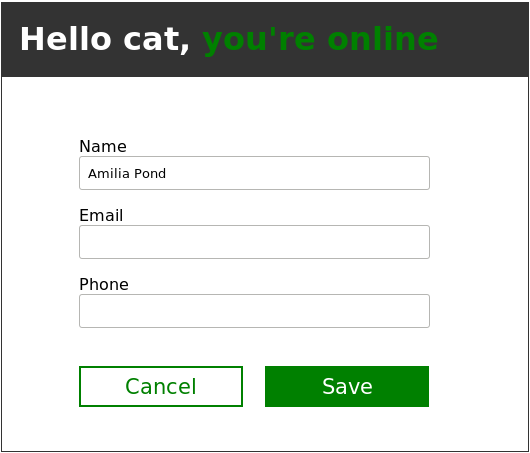
\includegraphics[width=\textwidth]{edit}
          \caption{Editieransicht im Onlinestatus}
          \label{fig:edit-online}
  \end{subfigure}
  ~ 
  \begin{subfigure}[t]{0.49\textwidth}
          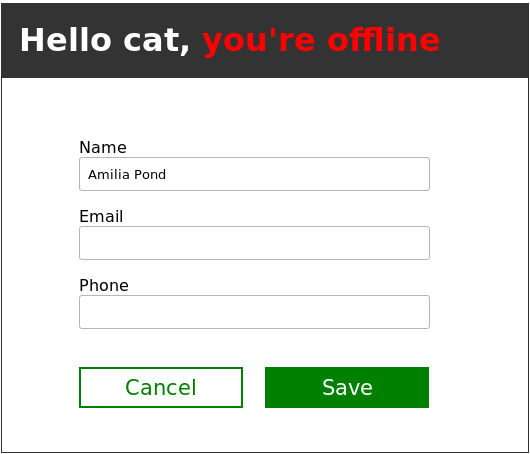
\includegraphics[width=\textwidth]{edit-offline}
          \caption{Editieransicht im Offlinestatus}
          \label{fig:edit-offline}
  \end{subfigure}
  \grayRule
  \caption{Die Editieransicht in beiden Netzwerkstatus}
  \label{fig:edit}
\end{figure}
Sobald ein Konflikt entstanden ist, soll sich ein Dialog öffnen, der die nutzenden Personen darüber informiert, welcher Kontakteintrag konfliktbehaftet ist und mit welcher Version er konkurriert.
Anhand des Dialoginhalts kann unterschieden werden, welche Version die lokal gespeicherte ist und welche vom Server kommt.
Der Dialog beinhaltet außerdem zwei unterschiedlich farbige Knöpfe, die jeweils den Kontakteintrag in einer anderen Version anzeigen.
Durch Klick auf einen Knopf wird die bevorzugte Version des Kontakts gespeichert und die andere verworfen.
So kann ein Mensch entscheiden, welche Version behalten werden soll und es wird sichergestellt, dass keine Daten verloren gehen.\\
Für die Implementierung des Konfliktdialogs ist es notwendig, dass die zu untersuchenden Technologien die Möglichkeit bieten, Konflikte zu speichern oder wenigstens als solche zu identifizieren, sodass sie manuell gespeichert werden können.
%
% Tests
%
\section{\label{chap:konzept:test}Testdurchläufe}
Um das Konfliktmanagement der zu testenden Technologien untersuchen zu können werden manuelle Tests durchgeführt.\\
Es müssen zunächst Konflikte erstellt werden, um zu untersuchen wie die verwendeten Technologien damit umgehen. Die zu entwickelnden Prototypen müssen auf mindestens zwei Geräten funktionieren und es muss die Möglichkeit bestehen den die Verbindung zum Internet oder zum Server zu unterbrechen.
Eine Variante Konflikte entstehen zu lassen ist, einen Kontakt an derselben Stelle zu bearbeiten während ein oder beide Geräte offline sind. Daher ist es wichtig zu wissen, in welchem Status sich die Anwendung befindet.
Die Testdurchläufe sind immer gleich und unabhängig vom Prototypen.\\\\
%Der genaue Ablauf eines Testlaufs sieht wie folgt aus.\\\\ 
Zuerst wird die \gls{App} in zwei Browsern gestartet. So kann die Verwendung von zwei Geräten simuliert werden. Da die Anwendung für die Browser Firefox und Chrome entwickelt wird, findet der Testdurchlauf auch in diesen beiden Browsern statt.\\
Es werden die Aktionen 'Kontakt anlegen', 'Kontakt bearbeiten' und 'Kontakt löschen' in unterschiedlichen Kombinationen und beiden Browsern durchgeführt.
In der ersten Testreihe sind beide Browser mit dem Internet verbunden und der Server ist an.
In der zweiten Testreihe wird ein Browser für eine Aktion vom Internet getrennt indem er in den Offlinemodus geschalten wird. Ist die Aktion in beiden Browsern abgeschlossen, wird der Offlinemodus des einen Browsers deaktiviert, sodass sich beide synchronisieren können.
In der dritten Testreihe wird der Server gestoppt, sodass beide Prototypen offline sind. Nachdem eine Aktion auf beiden Geräten vollständig durchgeführt wurde, wird der Server wieder gestartet und beide Anwendungen synchronisieren sich mit dem Server, oder der CouchDB.\\
Jede Testreihe wird einmal, in interschiedlichen Netzwerkstatus der Anwendung durchgeführt, pro Reihe gibt es drei bis vier Testdurchläufe.
In den Testreien eins und drei wird jeder genannte Testdurchlauf genau einmal durchgeführt.
Für die zweite Testreihe kann es, je nachdem in welchem Broswer die Aktion zuerst durchgeführt wird, unterschiedliche Ergebnisse geben.
Deswegen wird dort jeder Testdurchlauf zwei mal durchgeführt.
Einmal wird die Aktion in der Anwendung die mit dem Internet verbunden ist zuerst gespeichert, dann die im Offlinemodus.\\
Die folgende Tabelle veranschaulicht die durchzuführenden Testdurchläufe.
%
\begin{longtable}[c]{@{}
>{\columncolor[HTML]{CFFCC2}}l lllll@{}}
\toprule
    \multicolumn{1}{p{0.05\textwidth}}{\cellcolor[HTML]{cffcc2}\textbf{Nr.}}
    & \multicolumn{1}{p{0.2\textwidth}}{\cellcolor[HTML]{cffcc2}\textbf{Firefox online}}
    & \multicolumn{1}{p{0.2\textwidth}}{\cellcolor[HTML]{cffcc2}\textbf{Firefox offline}}
    & \multicolumn{1}{p{0.2\textwidth}}{\cellcolor[HTML]{cffcc2}\textbf{Chrome online}}
    & \multicolumn{1}{p{0.2\textwidth}}{\cellcolor[HTML]{cffcc2}\textbf{Chrome offline}}\\ \hline \noalign{\vskip 0.1cm}
\endfirsthead
\endhead
%
% 
  \multicolumn{1}{p{0.05\textwidth}}{\cellcolor[HTML]{cffcc2}\textbf{1a}}
    & \multicolumn{1}{p{0.2\textwidth}}{anlegen}
    & \multicolumn{1}{p{0.2\textwidth}}{}
    & \multicolumn{1}{p{0.2\textwidth}}{anlegen}
    & \multicolumn{1}{p{0.2\textwidth}}{}\\ 
  \midrule
  \multicolumn{1}{p{0.05\textwidth}}{\cellcolor[HTML]{cffcc2}\textbf{1b}}
    & \multicolumn{1}{p{0.2\textwidth}}{bearbeiten}
    & \multicolumn{1}{p{0.2\textwidth}}{}
    & \multicolumn{1}{p{0.2\textwidth}}{bearbeiten}
    & \multicolumn{1}{p{0.2\textwidth}}{}\\ 
  \midrule
  \multicolumn{1}{p{0.05\textwidth}}{\cellcolor[HTML]{cffcc2}\textbf{1c}}
    & \multicolumn{1}{p{0.2\textwidth}}{löschen}
    & \multicolumn{1}{p{0.2\textwidth}}{}
    & \multicolumn{1}{p{0.2\textwidth}}{löschen}
    & \multicolumn{1}{p{0.2\textwidth}}{}\\ 
  \bottomrule
  \bottomrule
  %
  \multicolumn{1}{p{0.05\textwidth}}{\cellcolor[HTML]{cffcc2}\textbf{2a}}
    & \multicolumn{1}{p{0.2\textwidth}}{anlegen}
    & \multicolumn{1}{p{0.2\textwidth}}{}
    & \multicolumn{1}{p{0.2\textwidth}}{}
    & \multicolumn{1}{p{0.2\textwidth}}{anlegen}\\ 
  \midrule
  \multicolumn{1}{p{0.05\textwidth}}{\cellcolor[HTML]{cffcc2}\textbf{2b}}
    & \multicolumn{1}{p{0.2\textwidth}}{bearbeiten}
    & \multicolumn{1}{p{0.2\textwidth}}{}
    & \multicolumn{1}{p{0.2\textwidth}}{}
    & \multicolumn{1}{p{0.2\textwidth}}{bearbeiten}\\ 
  \midrule
  \multicolumn{1}{p{0.05\textwidth}}{\cellcolor[HTML]{cffcc2}\textbf{2c}}
    & \multicolumn{1}{p{0.2\textwidth}}{löschen}
    & \multicolumn{1}{p{0.2\textwidth}}{}
    & \multicolumn{1}{p{0.2\textwidth}}{}
    & \multicolumn{1}{p{0.2\textwidth}}{löschen}\\ 
  \midrule
  \multicolumn{1}{p{0.05\textwidth}}{\cellcolor[HTML]{cffcc2}\textbf{2d}}
    & \multicolumn{1}{p{0.2\textwidth}}{bearbeiten}
    & \multicolumn{1}{p{0.2\textwidth}}{}
    & \multicolumn{1}{p{0.2\textwidth}}{}
    & \multicolumn{1}{p{0.2\textwidth}}{löschen}\\ 
  % \midrule
  %   \multicolumn{1}{p{0.05\textwidth}}{\cellcolor[HTML]{cffcc2}\textbf{2d}}
  %   & \multicolumn{1}{p{0.2\textwidth}}{löschen}
  %   & \multicolumn{1}{p{0.2\textwidth}}{}
  %   & \multicolumn{1}{p{0.2\textwidth}}{}
  %   & \multicolumn{1}{p{0.2\textwidth}}{bearbeiten}\\ 
  \bottomrule
  \bottomrule
  %
  \multicolumn{1}{p{0.05\textwidth}}{\cellcolor[HTML]{cffcc2}\textbf{3a}}
    & \multicolumn{1}{p{0.2\textwidth}}{}
    & \multicolumn{1}{p{0.2\textwidth}}{anlegen}
    & \multicolumn{1}{p{0.2\textwidth}}{}
    & \multicolumn{1}{p{0.2\textwidth}}{anlegen}\\ 
  \midrule
  \multicolumn{1}{p{0.05\textwidth}}{\cellcolor[HTML]{cffcc2}\textbf{3b}}
    & \multicolumn{1}{p{0.2\textwidth}}{}
    & \multicolumn{1}{p{0.2\textwidth}}{bearbeiten}
    & \multicolumn{1}{p{0.2\textwidth}}{}
    & \multicolumn{1}{p{0.2\textwidth}}{bearbeiten}\\ 
  \midrule
  \multicolumn{1}{p{0.05\textwidth}}{\cellcolor[HTML]{cffcc2}\textbf{3c}}
    & \multicolumn{1}{p{0.2\textwidth}}{}
    & \multicolumn{1}{p{0.2\textwidth}}{löschen}
    & \multicolumn{1}{p{0.2\textwidth}}{}
    & \multicolumn{1}{p{0.2\textwidth}}{löschen}\\ 
  \midrule
  \multicolumn{1}{p{0.05\textwidth}}{\cellcolor[HTML]{cffcc2}\textbf{3d}}
    & \multicolumn{1}{p{0.2\textwidth}}{}
    & \multicolumn{1}{p{0.2\textwidth}}{bearbeiten}
    & \multicolumn{1}{p{0.2\textwidth}}{}
    & \multicolumn{1}{p{0.2\textwidth}}{löschen}\\ 
  % end
  \bottomrule \cellcolor[HTML]{FFFFFF}
  \vspace{0.1cm}\\
  \noalign{\hspace{0.0525\textwidth}\grayRule}
  \caption{Testdurchläufe}
  \label{tab:konzept:tests}\\
\end{longtable}
%
%
%
Zur Auswertung der Tests werden alle Ausgangspositionen, Vorgänge und Ergebnisse dokumentiert werden.
Für einen Testdurchlauf wird hierfür der Kontakt und um welchen Testdurchlauf es sich handelt aufgeschrieben.
Außerdem wird festgehalten auf welchem der beiden Geräte die Aktion zuerst durchgeführt wurde, das erwartete und das tatsächliche Ergebnis.
